\documentclass[12pt,a4paper]{scrartcl} 
\usepackage[utf8]{inputenc}
\usepackage[english,russian]{babel}
\usepackage{indentfirst}
\usepackage{misccorr}
\usepackage{graphicx}
\usepackage{amsmath}
\begin{document}
	\begin{titlepage}
		\begin{center}
			\large
			МИНИСТЕРСТВО НАУКИ И ВЫСШЕГО ОБРАЗОВАНИЯ РОССИЙСКОЙ ФЕДЕРАЦИИ

			Федеральное государственное бюджетное образовательное учреждение высшего образования

			\textbf{АДЫГЕЙСКИЙ ГОСУДАРСТВЕННЫЙ УНИВЕРСИТЕТ}
			\vspace{0.25cm}

			Инженерно-физический факультет

			Кафедра автоматизированных систем обработки информации и управления
			\vfill

			\vfill

			\textsc{Отчет по практике}\\[5mm]

			\LARGE\textit{Вариант 3}

			{\LARGE Решение системы линейных алгебраических уравнений методом Гаусса}
			\bigskip

			1 курс, группа 1ИВТ АСОИУ
		\end{center}
		\vfill

		\newlength{\ML}
		\settowidth{\ML}{«\underline{\hspace{0.7cm}}» \underline{\hspace{2cm}}}
		\hfill\begin{minipage}{0.5\textwidth}
			Выполнил:\\
			\underline{\hspace{\ML}} Н.\,Д.~Ксенофонтов\\
			«\underline{\hspace{0.7cm}}» \underline{\hspace{2cm}} 2024 г.
		\end{minipage}%
		\bigskip

		\hfill\begin{minipage}{0.5\textwidth}
			Руководитель:\\
			\underline{\hspace{\ML}} С.\,В.~Теплоухов\\
			«\underline{\hspace{0.7cm}}» \underline{\hspace{2cm}} 2024 г.
		\end{minipage}%


		\vfill



		\begin{center}

			Майкоп, 2024 г.
		\end{center}
	\end{titlepage}
\LARGE{Содержание}

\begin{enumerate}
	\item Задача
	\item Пример кода, решающего данную задачу
	\item Скриншот работы программы
\end{enumerate}
\section{Задача}
Решение системы линейных алгебраических уравнений методом Гаусса.
\section{Пример кода}
\label{sec:exp:code}
\begin{verbatim}
#include <iostream>
#include <iomanip>
using namespace std;

int main() {
    setlocale(LC_ALL, "Russian");
    int n; // размерность системы
    double a[100][100]; // коэффициенты
    double b[100]; // свободные члены
    double x[100]; // решение
    // ввод размерности
    cout << "Введите размерность системы: ";
    cin >> n;

    // ввод коэффициентов и свободных членов
    cout << "Введите коэффициенты:\n";
    for (int i = 0; i < n; i++) {
        for (int j = 0; j < n; j++) {
            cin >> a[i][j];
        }
        cin >> b[i];
    }
    // метод Гаусса
    for (int i = 0; i < n; i++) {
        // выбор ведущего элемента
        int max_row = i;
        for (int j = i + 1; j < n; j++) {
            if (abs(a[j][i]) > abs(a[max_row][i])) {
                max_row = j;
            }
        }
        swap(a[i], a[max_row]);
        swap(b[i], b[max_row]);

        // прямой ход
        for (int j = i + 1; j < n; j++) {
            double factor = a[j][i] / a[i][i];
            for (int k = i; k < n; k++) {
                a[j][k] -= factor * a[i][k];
            }
            b[j] -= factor * b[i];
        }
    }

    // обратный ход
    for (int i = n - 1; i >= 0; i--) {
        x[i] = b[i];
        for (int j = i + 1; j < n; j++) {
            x[i] -= a[i][j] * x[j];
        }
        x[i] /= a[i][i];
    }
    // вывод результата
    cout << "Решение:\n";
    for (int i = 0; i < n; i++) {
        cout << "x[" << i << "] = " << setprecision(3) << x[i] << endl;
    }

    return 0;
}

	
	
	
\end{verbatim}
\vfill

\section{Скриншот работы программы}
\label{sec:picexample}
\begin{figure}[h]
	\centering
	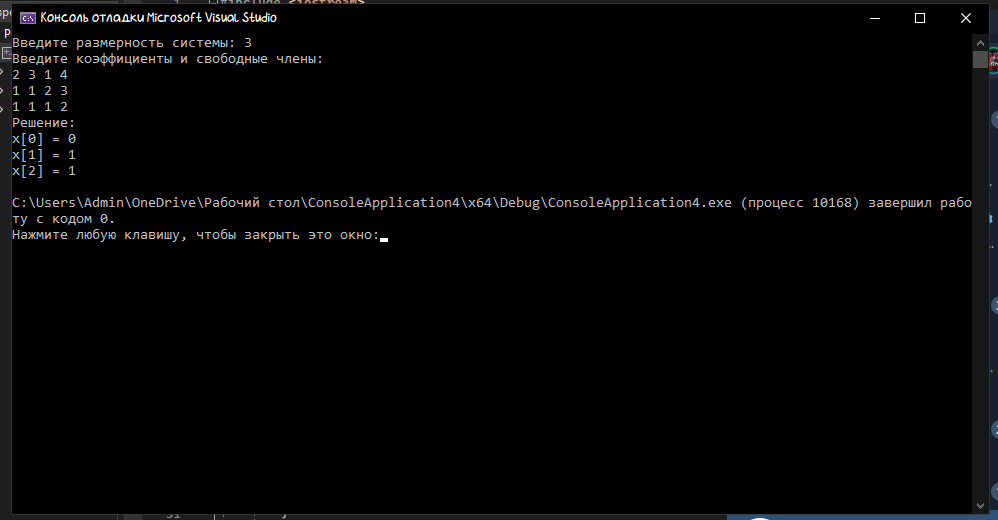
\includegraphics[width=0.9\textwidth]{pract.png}
	\caption{Результат}\label{fig:par}
\end{figure}
\end{document}